\documentclass[openany]{book}
\usepackage{latex/todonotes}
\usepackage{graphicx}
\usepackage{setspace}
\usepackage{booktabs}
\usepackage{latex/ulem}
\usepackage{geometry}
\usepackage{listings}
\usepackage{float}
%Tikz-UML Dependancies - pdflscape used to fix landscape sections in pdf export
\usepackage{pdflscape}
\usepackage{tikz}
\usepackage{ifthen}
\usepackage{xstring}
\usepackage{calc}
\usepackage{pgfopts}
\usepackage[english]{babel}
\usepackage[T1]{fontenc}
\usepackage{latex/tikz-uml}
\usetikzlibrary{calc,trees,positioning,arrows,chains,shapes.geometric,%
    decorations.pathreplacing,decorations.pathmorphing,shapes,%
    matrix,shapes.symbols}
\tikzset{
>=stealth',
  punktchain/.style={
    rectangle, 
    rounded corners, 
    % fill=black!10,
    draw=black, very thick,
    text width=10em, 
    minimum height=3em, 
    text centered, 
    on chain},
  line/.style={draw, thick, <-},
  element/.style={
    tape,
    top color=white,
    bottom color=blue!50!black!60!,
    minimum width=8em,
    draw=blue!40!black!90, very thick,
    text width=10em, 
    minimum height=3.5em, 
    text centered, 
    on chain},
  every join/.style={->, thick,shorten >=1pt},
  decoration={brace},
  tuborg/.style={decorate},
  tubnode/.style={midway, right=2pt},
  pil/.style={->, thick, shorten <=2pt, shorten >=2pt},
}


\onehalfspacing
\renewcommand{\chaptername}{} % Remove chapter numbering

\title{User Manual - Turtlenet\\Ballmer Peak}
\author{M. Chadwick, P. Duff, A. Senin}

\begin{document}
\maketitle
\tableofcontents

\chapter{General}
\section{System Overview}
Turtlenet is a purpose-built, privacy oriented social network, which demands zero 
security or technical knowledge on behalf of its users. It allows communication 
between users securely, via both a form of instant messaging, and creating posts 
to a series of walls.

What makes Turtlenet significant, is even its service operators are unaware of the 
content of messages. It is designed from the ground up that they can never have 
access, even if they wanted to. This resolves the most common security issues that
plague modern social media networks, an issue Turtlenet does not have.

\section{Contact}
Team contact information:
\begin{itemize}
\item p.duff@turtlenet.com
\item l.thomas@turtlenet.com
\item a.senin@turtlenet.com
\item l.prince@turtlenet.com
\item m.chadwick@turtlenet.com
\item l.choi@turtlenet.com
\end{itemize}

\chapter{Getting Started}
\section{Getting started}
Welcome to using Turtlenet!  Through the use of Turtlenet, you will experience
the ease of use and the practicality of communicating and socialising with your
friends, family, business associates or anyone else that you know through a
medium where your data is ensured to be protected.  This user manual has been
designed and written specifically to assist the users by providing detailed
description of all the various uses of the program.  Let's get started!

\section{System Requirements}
These are the minimum system requirements for Turtlenet:

\begin{itemize}
\item An internet connection
\item Any OS with a JRE (version 1.6.x or higher)
\item Any up-to-date browser
\end{itemize}

\section{Installing Turtlenet}
In order to install Turtlenet, you simply download ONE of the files from our
website:

www.turtlenet.co.uk/downloads.html

Most users will want to get the version that is without 'TOR' as unless you know
what that acronym stands for, you won't have it installed.  It is an external
piece of networking software which adds another layer of security, hiding your
IP address so people don't know where you currently are.

As the file is a Java Archive (JAR), you can put it in whatever folder you
choose - Turtlenet doesn't mind.  It will create the required files and folders
when it is running so just pick a pleasant home for the download.

\section{Running Turtlenet}
Now you have the client on your computer, you will need to run it.  People who
are familiar in using Java may be able to work it out but this section is here
for those who want to make sure that they are going to run it first time
correctly and without frustration.  Here is what you do:
\begin{enumerate}
\item Open Command Prompt (Windows) or your Terminal (*nix and OS X)
\item use 'cd' to get to where your Turtlenet client .jar file is.
      Windows users changing drive letters will need the '/D' parameter.
      e.g. 'cd /D D:\\TurtlenetFolder\\'
\item You will want to run the java command: \newline
      \textit{'java -jar turtlenet.jar'}
\end{enumerate}

If you managed to get to the downloaded client JAR file and ran that command,
you should have the back end of the Turtlenet client running.  All you need to
do now is open your preferred browser, or one of the suggested browsers if you
have more than one, and type \textit{'localhost:3141'} into your URL bar.

If the browser did not complain about anything and just worked, you should see
a Turtlenet banner.  If so, you have your client running successfully!

\section{The Turtlenet Interface}
Turtlenet comes with a simple interface that has the main menu, which has the
following sections:
\begin{itemize}
\item My Wall
\item My Details
\item Messages
\item Friends
\item Logout
\end{itemize}

\section{Account Creation}
The user is expected to create a new account when using Turtlenet for the first
time.  In order to create an account, enter a user name and a password, as well
as repeating your password into the confirmation box.  Once the user has 
created an account they will be logged into Turtlenet.  From here onwards, the
user can then add further profile details should they wish to. How to do so will
be explained under the 'Using the System' section.


\chapter{Using the System}
This section extends upon the fundamentals mentioned in the Turtlenet (TN)
general section.

\section{Creating an Account}
The 'General' chapter only briefly mentions creating an account so to make this
section complete as a 'go-to' resource for users it will also be mentioned here
too.

This is where your private communications begin.

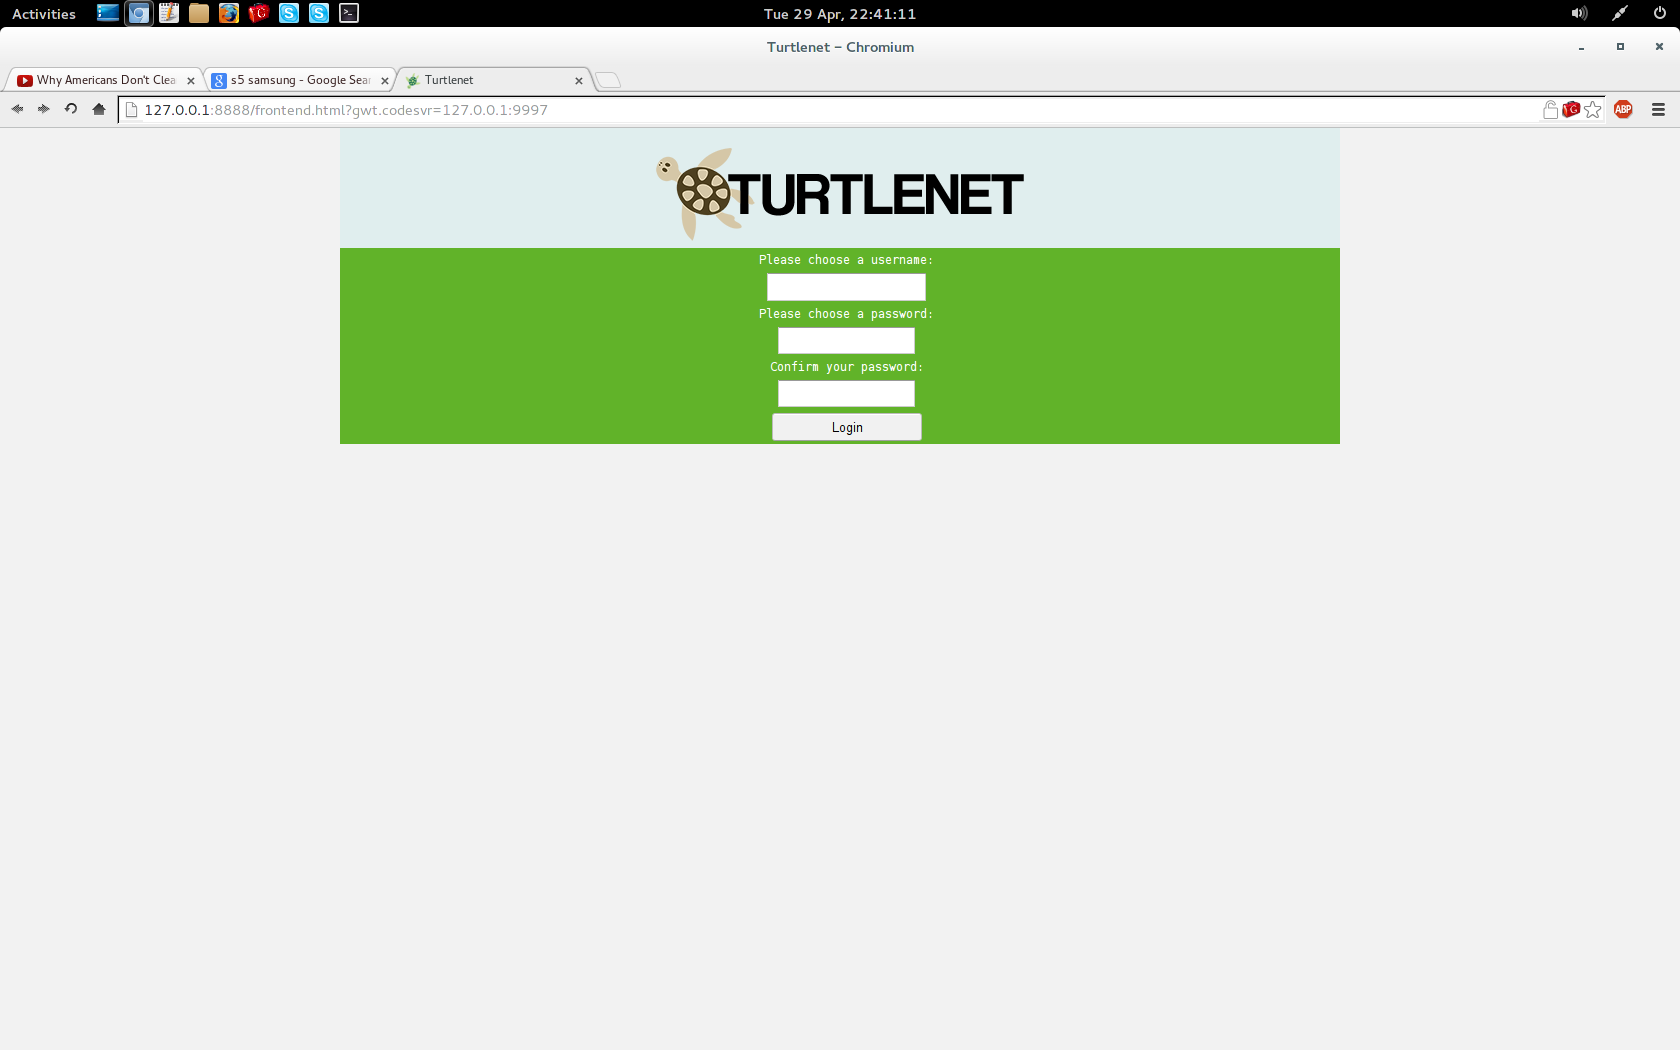
\includegraphics[scale=0.2]{screenshots/Screenshot from 2014-04-29 22-41-11}

This image shows the account creation page, which you should see when you run 
the client for the first time on your computer. From the top there are three
text boxes:
\begin{itemize}
\item a Username box
\item a Password box
\item a Confirmation box
\end{itemize}

You fill in each of the fields with the required information which will be the
following:
\begin{itemize}
\item The Username box should be filled in with your user name. This is what
      other users would call you when posting messages. This should be 
      something that represents you, but should not link to you outside of
      Turtlenet. Simply, your Turtlenet user name should not be the same as
      any other user name you use on the internet. If the name can be linked to
      you then people are able to easily determine that you have a turtlenet
      account.
\item Your password should be easy to remember but difficult for
      anyone else to guess. A good method for coming up with new passwords is
      to use four or five words, in a phrase. An example would be
      'ThisIsTurtlenetzPassword'. This is better and easier to remember than
      what is usually suggested which is a shorter password with numbers in
      them: 'P@ssw0rd'. Of course, it depends on who is remembering the
      password so choose your own method if either option mentioned feels
      uncomfortable for you.
\item The Confirmation box is where you type the password you defined in the
      previous box. Because of this, they should match, and must if the account
      creation is to be successful. The easiest way of thinking about this box
      is that it is giving you the practice of inputting your password while it
      is still fresh in your mind, to help you remember for later on.
\end{itemize}

By filling in these text boxes with the kind of information mentioned in this
section, you can then click the button underneath these boxes to create your
account. If successful you will be automatically logged in.

\pagebreak
\section{Logging into Turtlenet}
Logging into the Turtlenet client is as simple as using the password that you
had used to create your account.

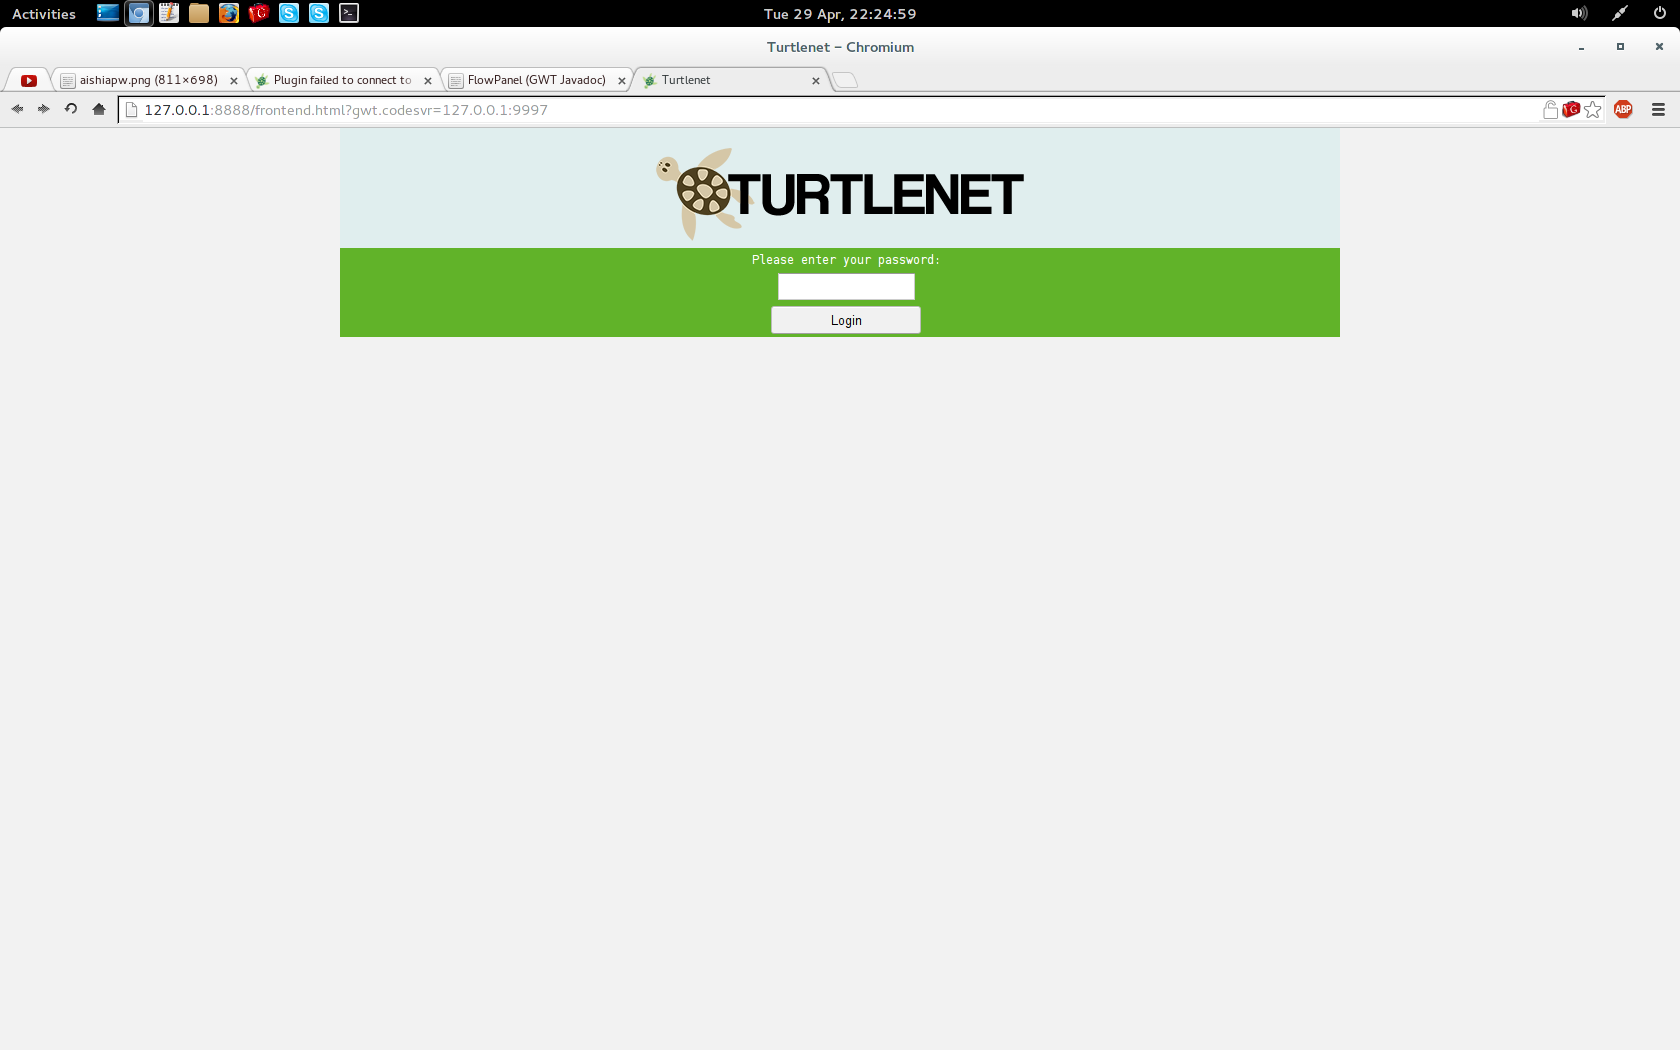
\includegraphics[scale=0.2]{screenshots/Screenshot from 2014-04-29 22-24-59}

The screen shot shows the initial page you might see once you have created an
account. Enter your password into the white text box above the 'Login' button
and if the password is correct, you would have logged in.

\pagebreak
\section{Navigating around the Turtlenet client}
Getting around the client's various areas is important in order to make the most
of the functionality provided by Turtlenet. This is why all of the main
segments are provided as buttons at the top of the interface:

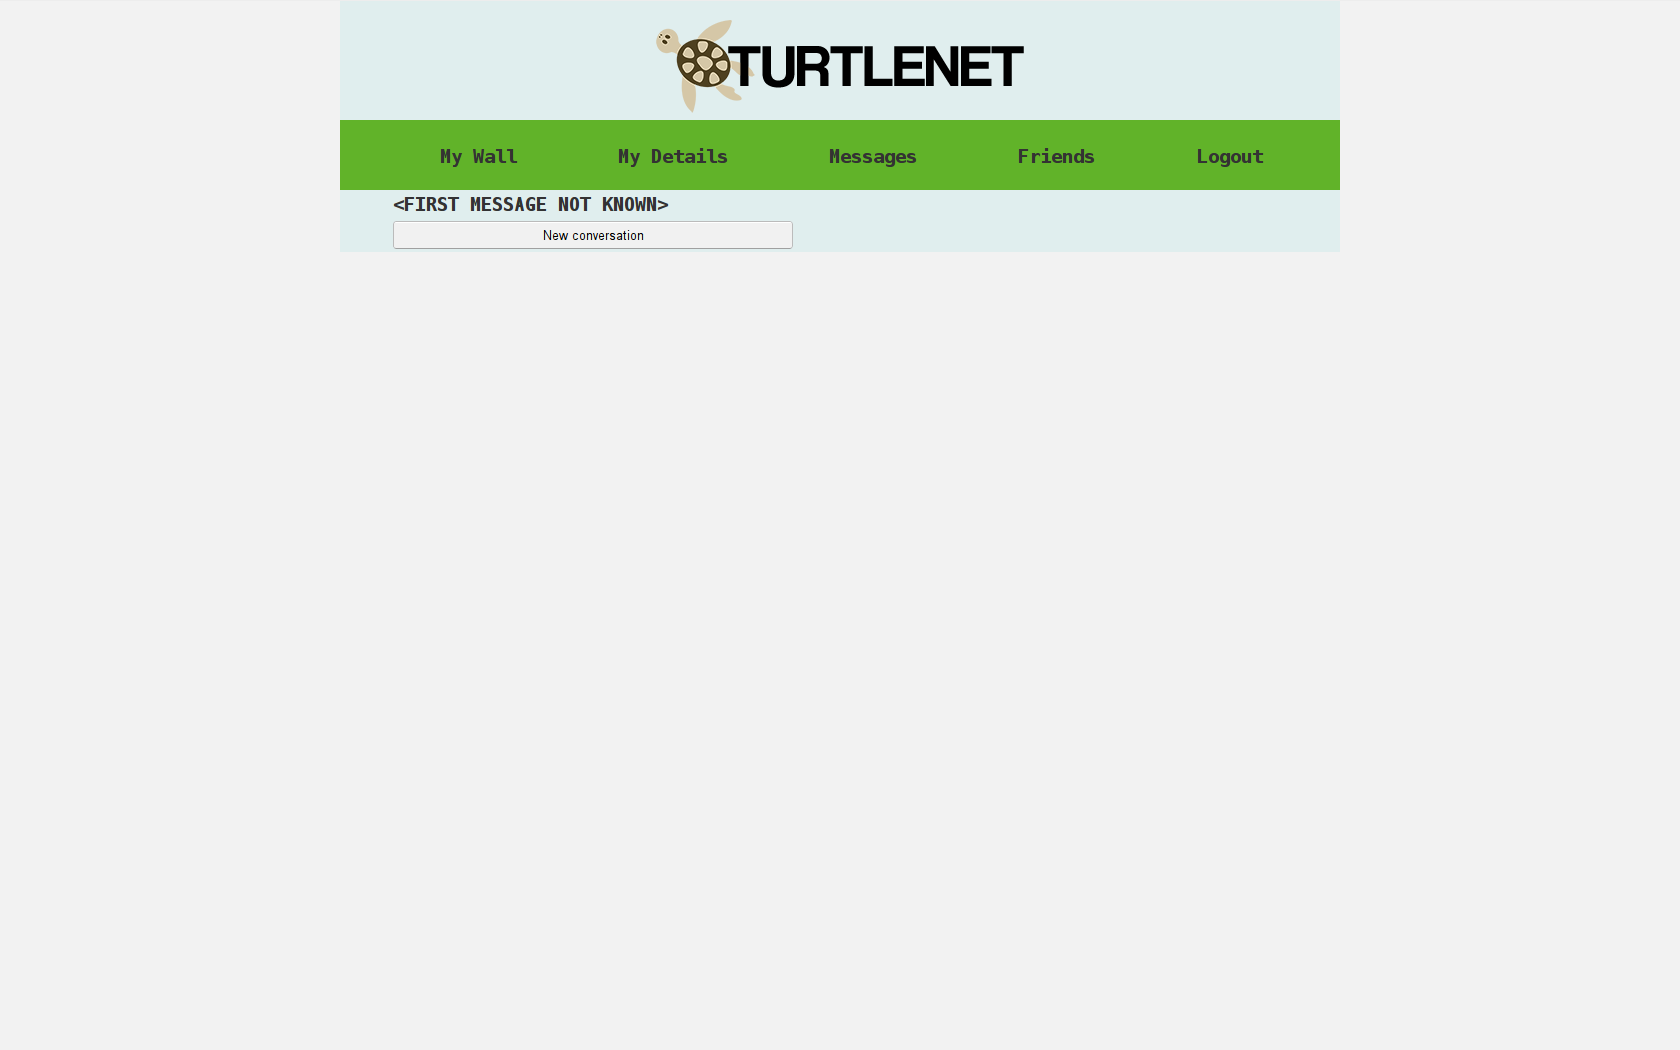
\includegraphics[scale=0.2]{screenshots/Screenshot from 2014-04-29 22-31-38}

The image shows that there are several main sections to the client - The wall,
the user's details, messages between the user and other people, friends that the
user has linked with and finally the function to logout. Click the
corresponding button to get to the area you wish to view. The following
sections will go through each section from right to left.

\section{Logging out}
For when you decide that you want to leave the safety of Turtlenet and work on
other things, or you simply need to be away for a while and want to be sure that
no one is using your account, you will want to log off. It is as painless as
clicking the 'log off' button found at the top right of every page. Doing so
will take you to the login screen (the one with just the password box and login
button). Of course, we wish you good fortune until you come and join us again
at Turtlenet.

\pagebreak
\section{Friends on Turtlenet}
Part of the philosophy of Turtlenet is to encrypt the messages that you send so
that only the intended recipients can read them with any understanding. These
people are known as your 'friends' on Turtlenet. In order to make any use of
Turtlenet you need to add friends. You do this by exchanging 'public keys' with
another user. Turtlenet uses Asymmetric relationships - this means that you may
have some people as friends but they might not have you as a friend. Therefore
you might understand what people have typed but they might not be reciprocated.
If this doesn't make sense at the moment, the following sections will help.

\subsection{The 'Getting'}
In order to get public keys from other users, they need to pass the information
to you.The keys can be transfered in any manner, they are not remotely private
and painting your public key on the side of your house would not diminish
security.

Once you have the public key off of your friend, you will want to proceed to the
'friends' section of the Turtlenet client, by clicking the button near the top
which has 'Friends' written upon it. You should either see the following or
something to it's effect:


\includegraphics[scale=0.2]{screenshots/Screenshot from 2014-04-29 22-31-10}

As you can see, there is 'My Key' which will be used by you to allow others to
send you messages but that will be explained in the next section. For now, you
want to click the 'Add new friend' button located to the right of the screen.
This will bring you to a screen with a long input box which asks for the key of
who will become your friend. You enter the long line of letters and numbers
that you were given by your friend into the input box. Once you have the other
person added, you should see something similar to this:


\includegraphics[scale=0.2]{screenshots/Screenshot from 2014-04-29 22-31-10}

In the image above, the current user has added themselves to their friends list.
Simply repeat the process as it takes you back to the main section for the
friends tab.

\subsection{The 'Making'}
By getting other people's keys you can send messages to them but for people to
send anything back that you can read, they would need to have your key as well.
All you do in order to help others add you is to send the letters and numbers
in the text box next to 'My key' and get the other user to follow the steps in
the above section 'The 'Getting'.'

\subsection{Banding Together}
In Turtlenet you can associate other users with categories, custom made by you.
This is useful if you want to send the same message to a number of people.
To do this, whilst you are in the friends section of the client, click the 
'Create category' button on the right. It should take you to this screen:

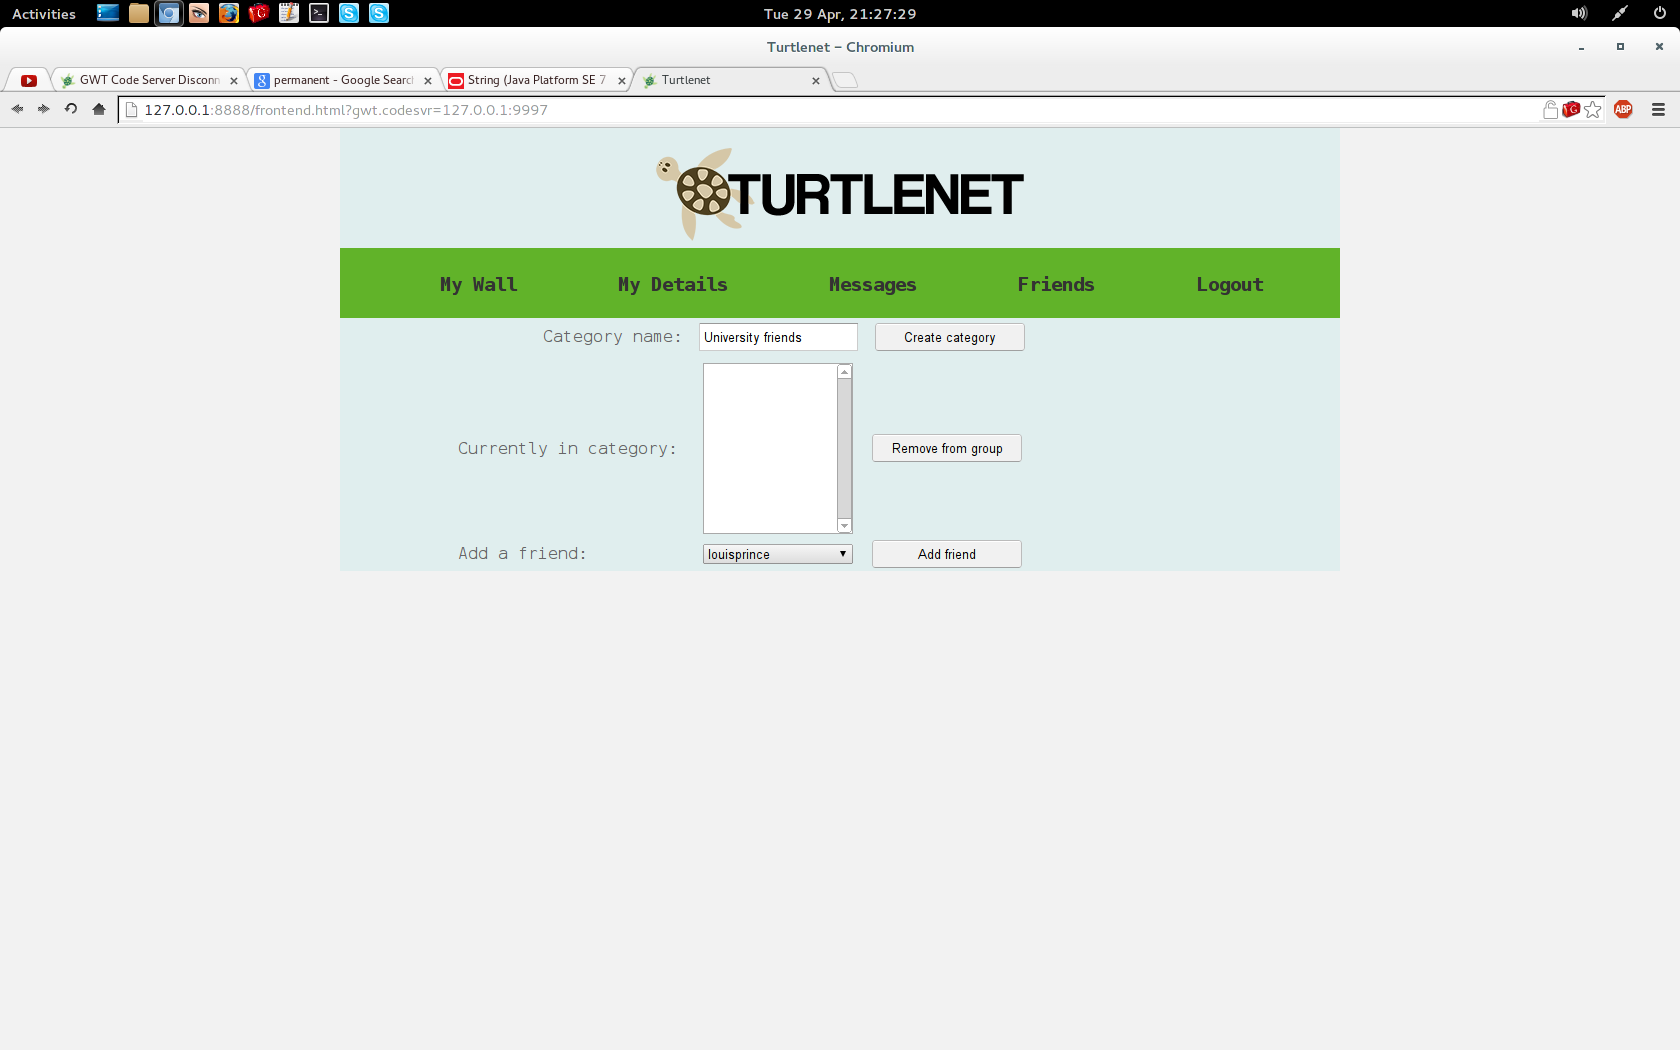
\includegraphics[scale=0.2]{screenshots/new6}

You will give your category a name so it hints to the kind of users you have in
them together by typing the group name in the top text box. Click 'Create
category' once you have finished the naming procedure. You are then able to add
any members you wish whose keys you have attached to your account. This is done
in the drop-down menu at the bottom of the interface and then clicking the 'Add
friend' button next to said menu. If you no longer want a particular user in
the group any more, select their user name in the large box in the middle and
click the button to the side which says 'Remove from group'.

\pagebreak
\section{Messages in Turtlenet}
Messages can be sent to singular users or they can be sent to categories of
users created by the current user of the client. Below is an example of what
you may find in the messages section:

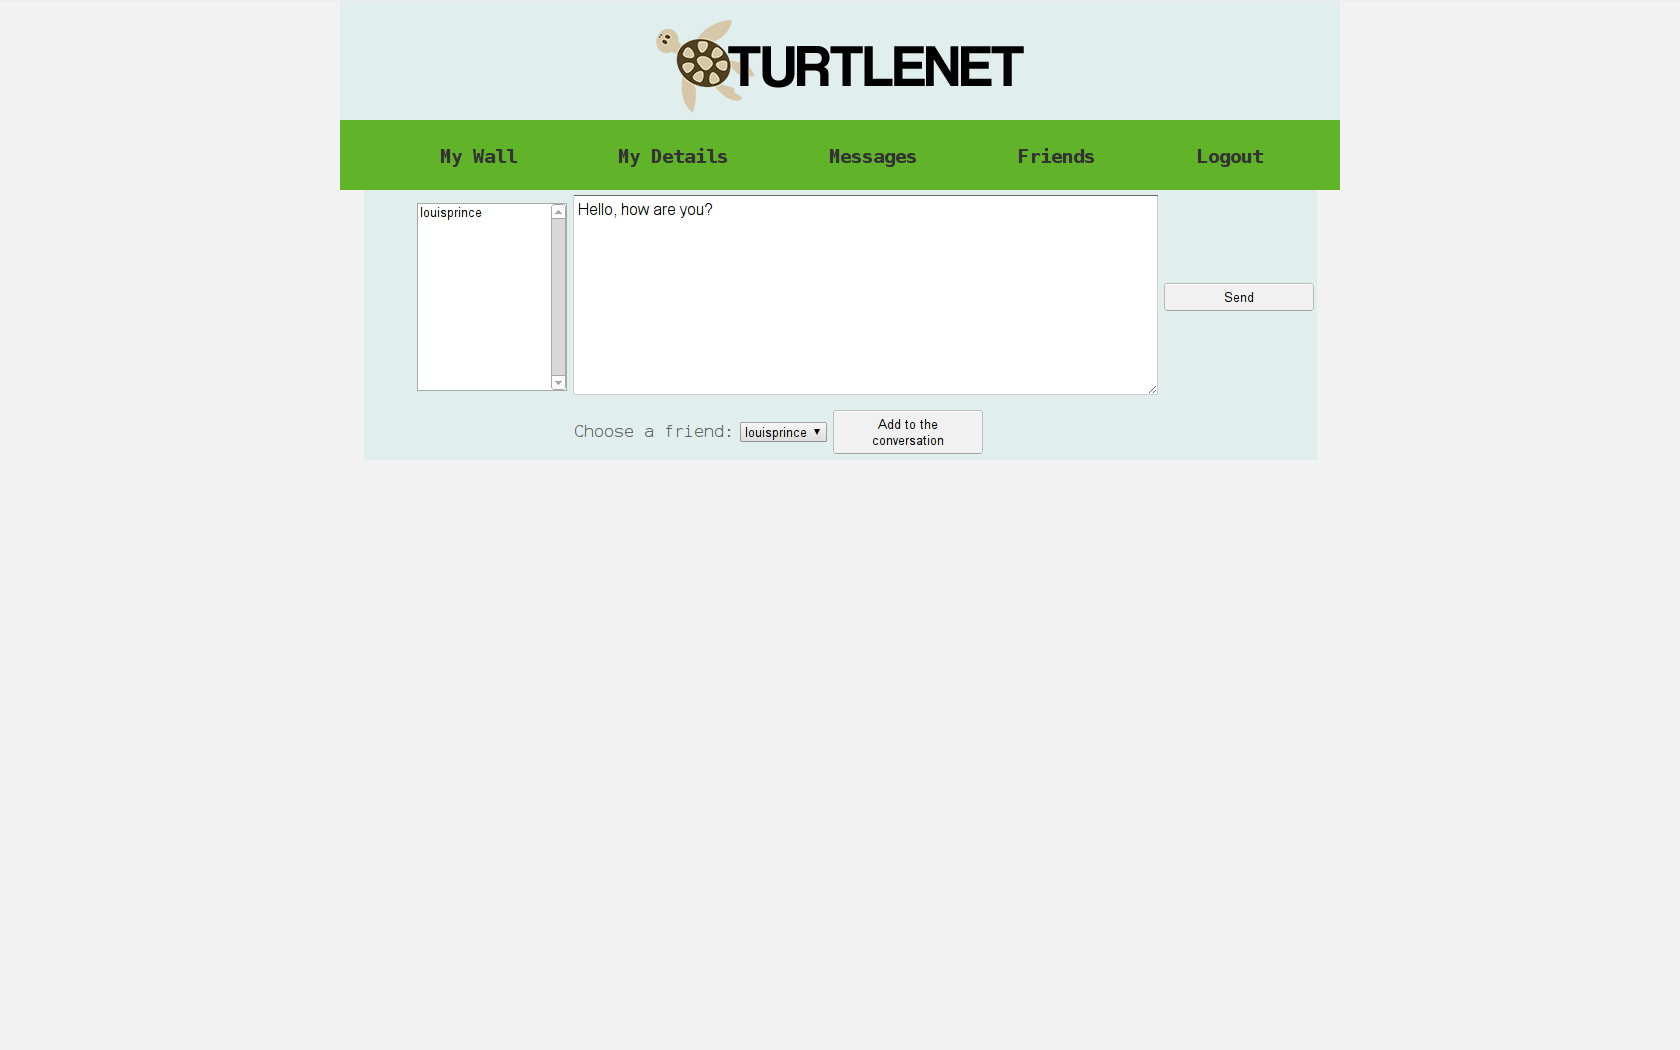
\includegraphics[scale=0.2]{screenshots/Screenshot from 2014-04-29 22-30-50}

\begin{itemize}
\item the box at the left hand side is for your available recipients - our
      example user only has himself at the moment. This will fill up over time
      when you add public keys from other users.
\item The larger of the two boxes is where you type the content of your message.
      There is no size limit.
\item The Send button on the right finalises the message and sends it to the
      recipient to read. You cannot edit your message once you have sent it
      so be sure to re-read what has been typed to avoid any unfortunate errors!
\end{itemize}

\section{What's mine is mine - Personal Data}
When using Turtlenet, personal data is just that - personal. Similar to all of
the messages and posts you make, your personal data is also encrypted and made
secure so that the server moderators have no access to them. Here is a view at
what you could see when entering the 'My Details' section of the client:

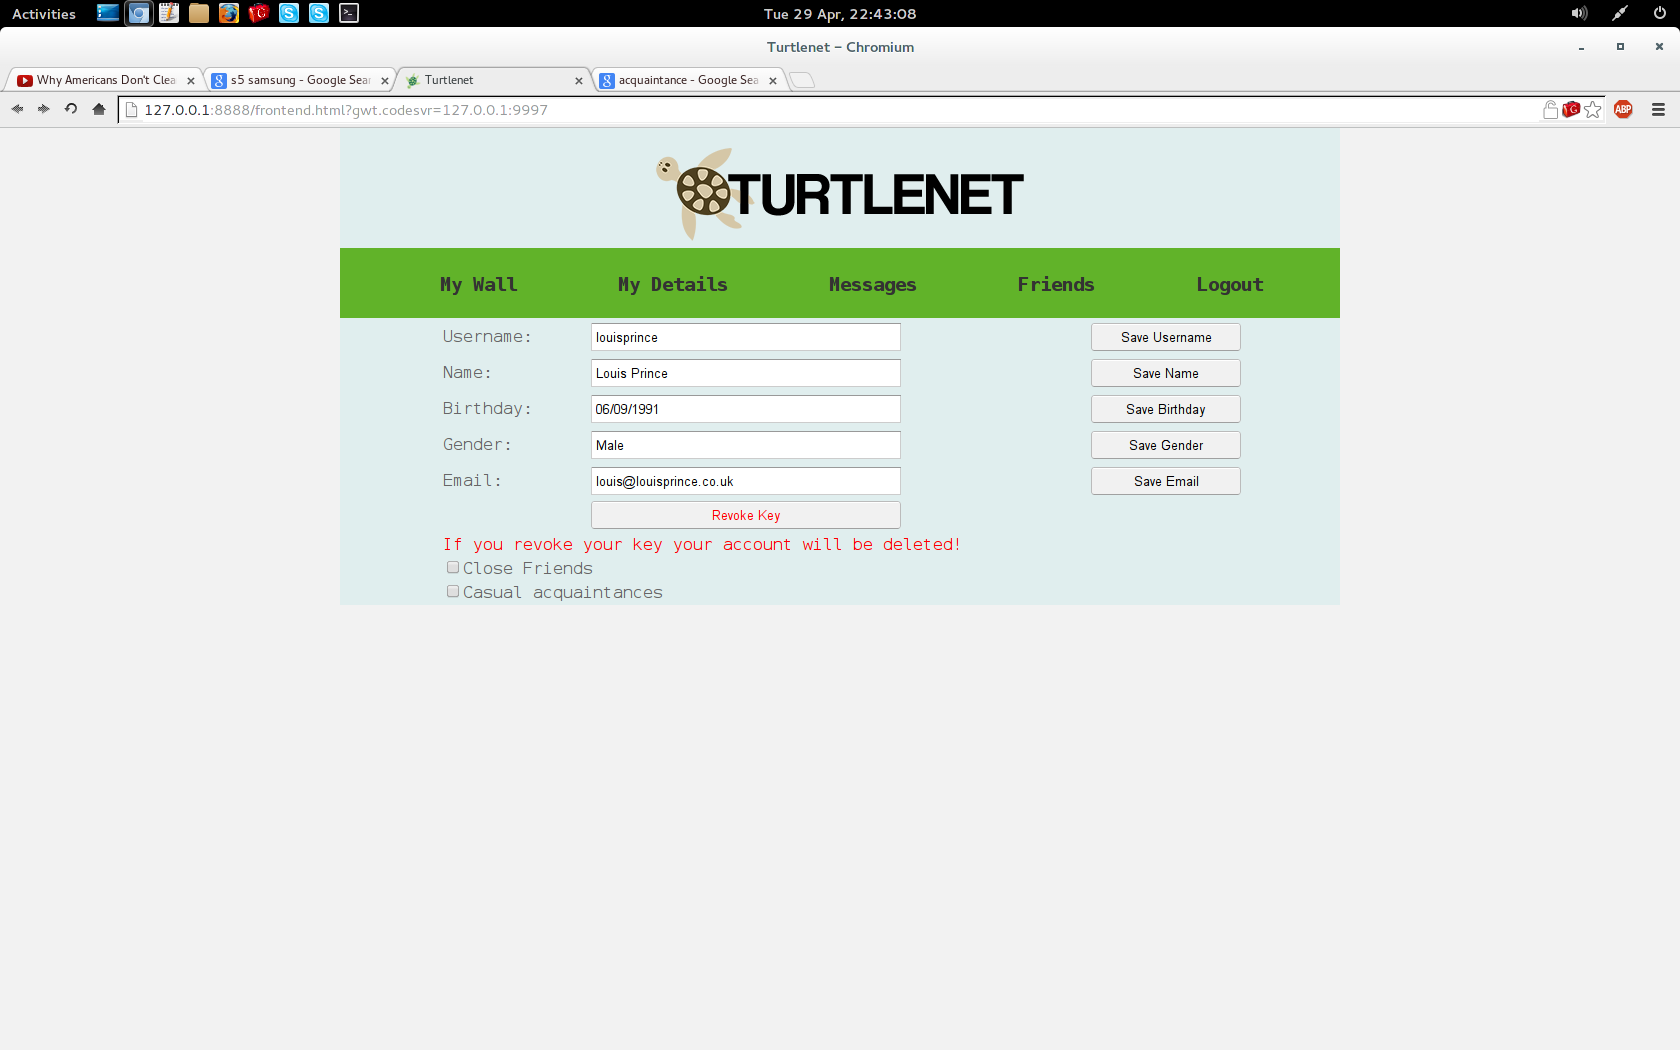
\includegraphics[scale=0.2]{screenshots/Screenshot from 2014-04-29 22-43-08}

The image shows the only personal information that you may store using the
Turtlenet client. Note that the only piece of information here that is 
important is the user name - all other fields are optional and at the user's
discretion to fill in or not. Each button to the right saves what is currently
in the associated field at the time of clicking, so you will need to save again
if you edit after a save.

Below these fields is a list of categories you have created, check the box next
to a category and members of it will be able to see your personal data.
Unchecking the box hides any futures changes in it from them.

A note about revoking your key:  This means that you mark your key as never
again to be trusted, and so messages from it are ignored.
\textbf{Do not click unless you wish to erase your Turtlenet presence.}
After a revocation, another key is made for you to use, which means that any other
users that had your key will need to be informed that you have changed and you
will need to give them your new key if you wish to continue getting messages 
and posts from them.

\pagebreak
\section{Personal Graffiti - your Turtlenet wall}
Your wall is a central social hub for many users of Turtlenet. It is a
collection of messages aimed at the user, who may be off-line at the time.
This section is for the functionality of the wall.

In Turtlenet a post is the generic way of talking about a message being left for
another user - think of it similar to a sticky note on a cork board.An example
of a wall is below:

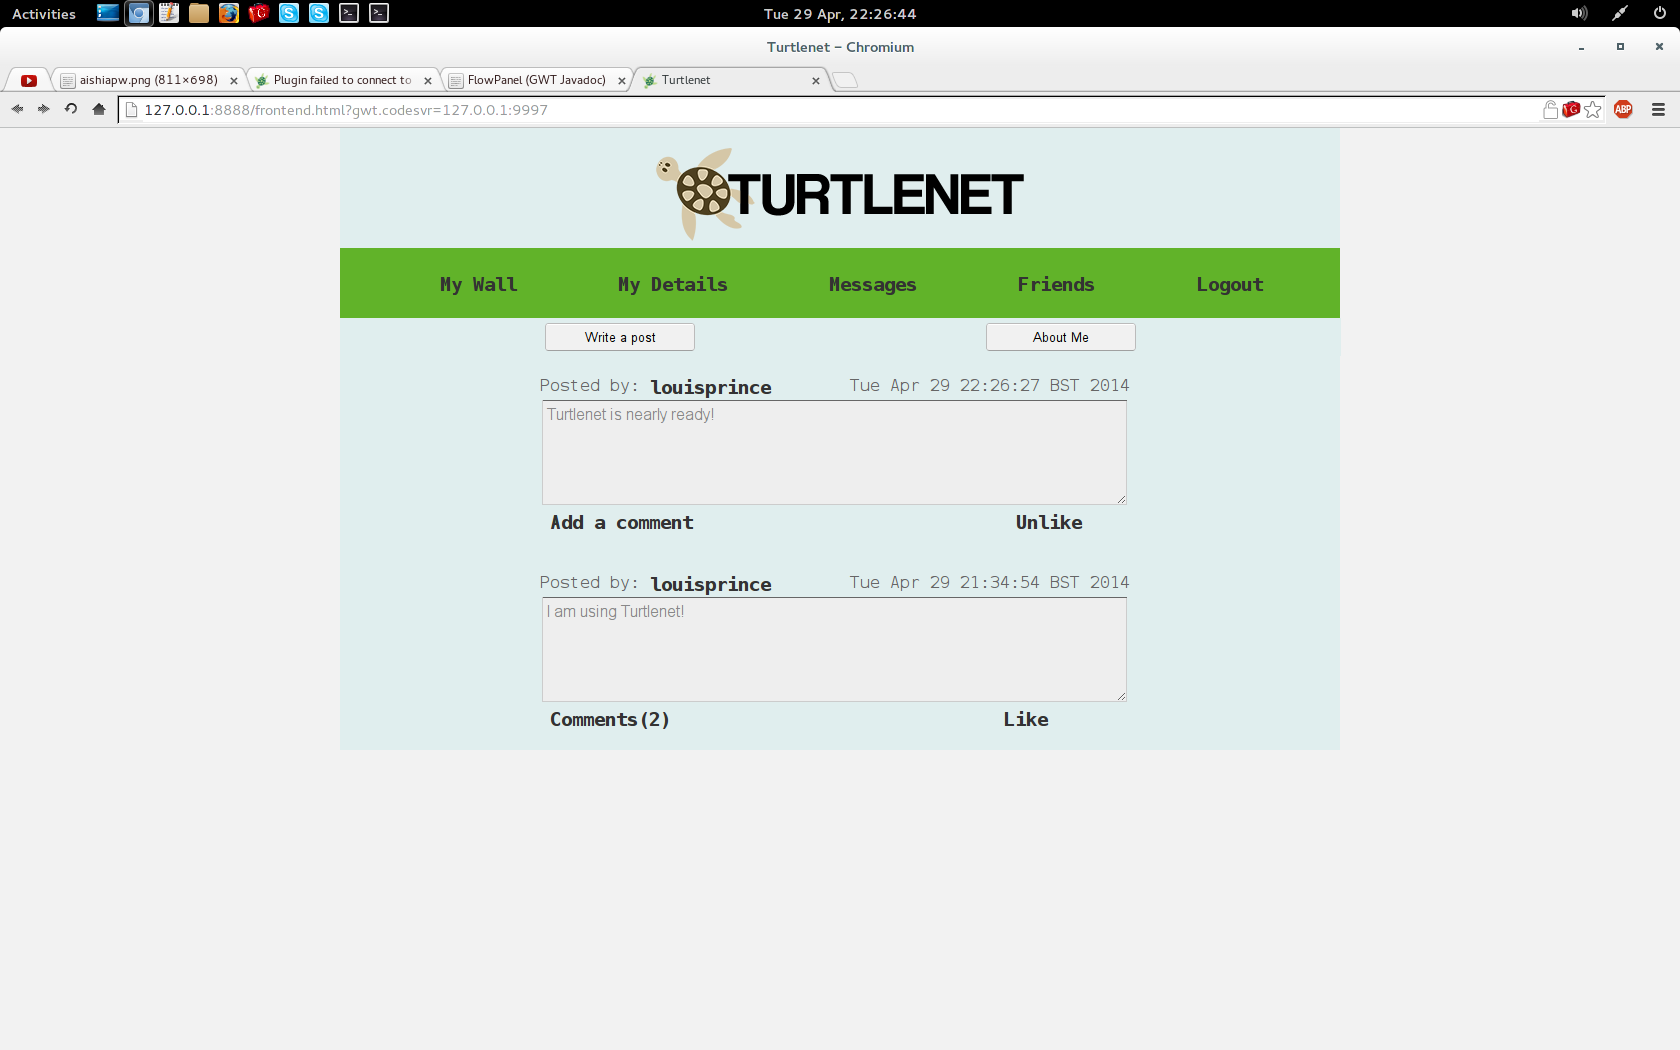
\includegraphics[scale=0.2]{screenshots/Screenshot from 2014-04-29 22-26-44}

The image outlines a couple of posts being made by the example user. Before 
posting is explained, this manual will explain the other elements in view:

\begin{itemize}
\item The 'About me' button allows a user to see an overview of their personal
      data. This allows a user quick access to their key, which could be sent to
      another user.
\item You can 'like' posts to show enjoyment, appreciation or agreement with
      what another user has posted. This is done by simply clicked the 'like'
      that is found underneath the target post. Should your political views
      change for example, you can unlike any currently liked post in the same
      manner - clicking the 'unlike' that will be found in the same place under
      the target post.
\item Commenting on a post is also possible with the Turtlenet client. Simply
      click the 'Add a comment' phrase underneath the target post and a large
      input box will appear beneath. Simply type your 'two cents' then click
      the 'Post comment' button under the input box. If you decide not to
      insert an interjection then you may click the Cancel button to remove the
      box and not attach your comment to the post.
\end{itemize}

Posting is as simple as clicking the 'Write a post' button near the top, which
will bring a couple of new elements into the client:

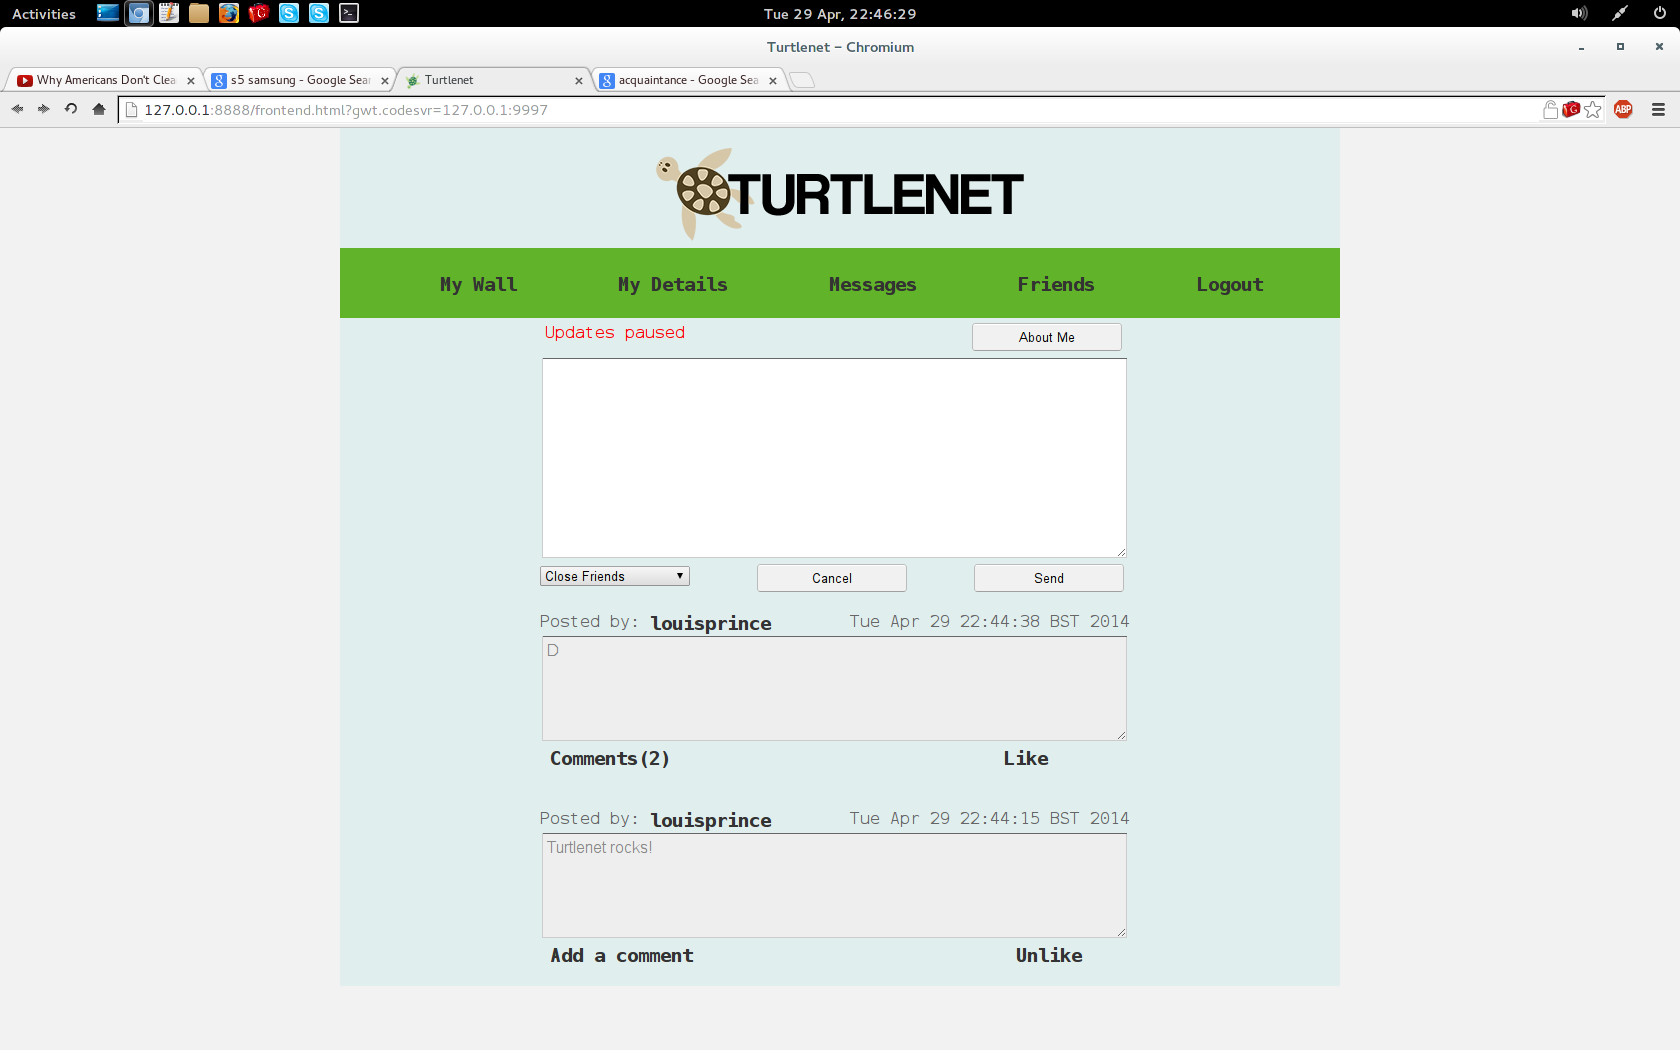
\includegraphics[scale=0.2]{screenshots/Screenshot from 2014-04-29 22-46-29}

As the above image shows, there are a couple of new buttons and a large text box
that appears onto the Turtlenet client. First it is easiest to define a target
for the post, which is done by clicking the drop down menu below the input box
on the left side. The user is able to choose from categories
that have been created, sending the post to multiple users. Once decided, type
the content of the post into the large input box. Once finished, click the
'Send' button below the input box on the right side. If you wish to stop
making a post, click the Cancel button in the middle, underneath the input box.


\chapter{Troubleshooting}
\section{Frequently Asked Questions}
This is the section which should hopefully answer most of the questions that
most users might have about the system.  Sending emails to one of the addresses 
in the contact section in the beginning of the user manual may help you get your
answer but it is best if you continue looking for an answer whilst you wait for
an official reply.

\subsection{What does Turtlenet do?}
Think of Turtlenet in a similar manner to any other social network commonly in
use.  It allows users to communicate with each other and allowing other people
to voice their opinions on what others have written.  At the moment it is text
based, meaning you can't attach images and video to it when you post or comment.
You can however send Universal Resource Links (URL) to each other, as they are
text based.  That is a convenient enough work around for the time being as it
means that no one is having to download an encrypted video but are never able to
view it as they do not have the key to unlock the data.  I think everyone will
appreciate not having current top 40 stored for a long time.

\subsection{How many accounts can I have on Turtlenet?}
As many as you like!  If you wish to have different personae within Turtlenet to
help filter friends from "It's kind of tricky I like them but they can be 
annoying" people then by all means - it's not on our head if they catch you 
putting them in the unmentionables list.

\subsection{I forgot my password.  Can someone reset it for me?}
The short answer is no.  Turtlenet was designed so that no one but the user had
access to personal data, protecting them from unwanted external influences.  As
a result, if you lose your password we are unable to recover anything in the
account.  The only thing you can do is simply to create another.  Feel safe in 
the knowledge that everything is encrypted on your old account so at least no 
one can access what was lost.

\subsection{Where is everything stored?}
On your computer, laptop or whatever else it is that uses the Turtlenet client.
Each client downloads all of the data and reads what it can, using keys you have
collected over time off of other users.  Keeping it local means that nothing is
stored on the server, so evil moderators cannot have their way with your data.
This also means that your data is stored on someone else's device but don't worry
 - just as you cannot read that user's information they cannot read yours.

\subsection{How big does this database get?}
As the only things being stored are text, not images or video, this means that
each message is only small and could only be about 4-8 gigabytes (GB) over one
year's use.  Bear in mind that the database is a replica of the entire history
of Turtlenet, along with everything every user has ever posted and commented on.
so much data for such a small size is pretty good.  In this time the project may
also have development applied to it, either from the original developers or the
community, so a cleaning function may be added to a future release.  We don't 
know.

\subsection{Why would someone want to build from source?}
For computers using Linux especially, the pre-built files may not work on their
system so in order to use Turtlenet, they would have to build the client
themselves.  Most Windows and Mac OS X users won't have to worry about this,
although if they want and know what to do, they are welcome to try!

\subsection{The Client does stuff I don't think it should do...}
You may have found a bug for us accidentally.  email to one of the addresses at
the beginning of the user manual and the developers will have a look at it.  As
the source is being released, maybe the community will have a look and suggest a
fix themselves.

\subsection{What do Server Moderators of Turtlenet do?}
Most of the time they watch text that they cannot understand go across the
screen.  This is to make sure that the server doesn't stop for some unknown 
reason.  They don't actually have any knowledge about what is being sent between
users so encode mildly evil messages and they will be none the wiser.  Unless
they have logged in as a user as well as moderating.  Then they still won't know
everything unless everyone adds the moderator's 'user account.'  A need-to-know
basis is what Turtlenet achieves.

\subsection{I want to mod Turtlenet.  Can I have the source?}
It's nice to know that others wish to take up the helm, pioneering a secure 
method of communication.  You can have the source, it is available to the public
to browse and modify.  One of the tools used in the initial development uses a
version of the GNU GPL, so be aware of what you can and can't do because of the
copyleft licence when you modify and distribute the project and it's source code.

\subsection{Why choose 'X' over the clearly superior 'Y'?}
As developers ourselves, we understand that other people have differing opinions.
That's the joy of releasing code.  Other people can pick up what we have done,
or use our ideals as a starting point for their own thing.  What this project
stood for is ease of use for the end user and security from any unwanted external
influences and this, we believe, is achieved.

\end{document}
